% =========================================================================
% CHAPTER 8 — EVALUATE: THE USER STUDY
% =========================================================================

\chapter{User Study}
\label{ch:userstudy}

\noindent
{\rmfamily\itshape
\begin{tabular}[t]{@{}l@{\hspace{0.3cm}}p{12.5cm}@{}}
\textls[50]{\textbf{Addressed:}} &
\textls[50]{Testing \& Validation · Between-Subjects Design · Survey Instrument · Written
Comprehension Protocol · Coding Framework · Consent \& Ethics · Design Limitations}
\end{tabular}
}

\vspace{0.5cm}

Chapter~\ref{ch:translate} developed the artefact and showed that the two conditions contain the same information. The next question is whether presenting this information in different ways affects how people understand it. This chapter describes the user study designed to investigate this question. The study does not aim to prove that experiential visualisation is better. Instead, it examines whether a small group of mostly non-specialist participants understands the system differently when presented with a static or an experiential visualisation. The study is also designed so that both positive and negative results can provide useful information for the next stage of the research. It is a \emph{socio-cognitive study}, aimed at understanding how people interpret the visualisations rather than at testing the underlying science or the competence of the participants.

% -------------------------------------------------------------------------
\section{Purpose}
\label{sec:eval-purpose}

Chapters~\ref{ch:data_pipeline} and~\ref{ch:translate} addressed the detection and translation stages. The remaining step was to put the two forms of representation in front of participants and compare how they understand them, which is what the central research question (\S\ref{sec:rqs}) asks. A \emph{comparative user study} was therefore required. Because animated visualisations can appear more effective than static ones simply by carrying information the static version lacks \citep{tversky2002}, the study holds the underlying information constant between conditions and varies only how it is presented.

% -------------------------------------------------------------------------
\section{An Exploratory First Stage}
\label{sec:eval-exploratory}

The study is exploratory by design. Twenty-five participants took part, twelve assigned to the static condition and thirteen to the experiential.\footnote{The difference between twelve and thirteen follows from random assignment at a small sample size. It affects nothing in the descriptive analysis beyond the denominators used in Chapter~\ref{ch:results}.} A sample of this size is not sufficient for broad inferential statistics or population-level generalisation, and the study makes no such claims.

The sample size was set a priori, on grounds of feasibility and of the exploratory aim, rather than determined during data collection --- and it is worth being explicit about what does and does not justify it. A saturation criterion, continuing until new responses stop yielding new categories, is not claimed and would not be appropriate: saturation belongs to inductive, theory-generating designs, whereas this analysis is deductive against a grid fixed before the responses were read, and the responses were collected in full before coding began \citep{braunclarke2021}.

The defensible criterion is \emph{information power} \citep{malterud2016}: the number of participants a qualitative study needs falls as its aim narrows, its sample becomes more specific, its theoretical grounding strengthens and its analysis works across categories rather than within cases. This study is narrow in aim, specific in sample, grounded in a coding grid derived from the design grammar of Chapter~\ref{ch:literature}, and analysed by category across participants. Twenty-five participants carry adequate information power for that configuration, and none for the population-level inference the study does not attempt.

The purpose of this first study is instead to identify initial patterns that can inform future research: which concepts participants understand, which are commonly misunderstood, whether the two conditions appear to lead to different interpretations, and whether the approach is promising enough to justify a larger and statistically powered study. It is a first empirical step, not a final test of the proposed approach.

% -------------------------------------------------------------------------
\section{Participants and Audience}
\label{sec:eval-audience}

The study targeted non-specialists: participants without specific training in oceanography, climate science, mathematics or machine learning. Non-specialist status was established by self-report in the background section. This choice directly reflects the aim of the thesis. The visualisations are intended to support the understanding of complex systems beyond specialised scientific audiences.

Participants were not expected to have prior knowledge of the AMOC or of the concepts used in the visualisations; the survey provided the basic information needed to approach the scenes. Recruitment ran through personal networks in Italian and English, so the sample is a convenience sample: its composition is described in \S\ref{sec:eval-demographics} and its implications in \S\ref{sec:eval-limitations}. This matters for the design. If a visualisation can only be understood by people who already know the system, it does not address the communication problem this thesis is about.

% -------------------------------------------------------------------------
\section{The Instrument}
\label{sec:eval-instrument}

Due to its exploratory nature, the study was conducted as a self-guided written survey using Google Forms. Four versions of the survey were used, combining two languages (Italian and English) with the two experimental conditions (static and experiential).\footnote{The four forms use the same wording within each language and differ only in the scene links leading to the static or experiential visualisations. The complete survey protocols are provided in Appendix~\ref{app:protocols}.}

% ============================================================
% fuse* Artificial Botany (2019) -- original figure
% extracted from the studio's website.
% ============================================================

\begin{figure}[htbp]
    \centering
    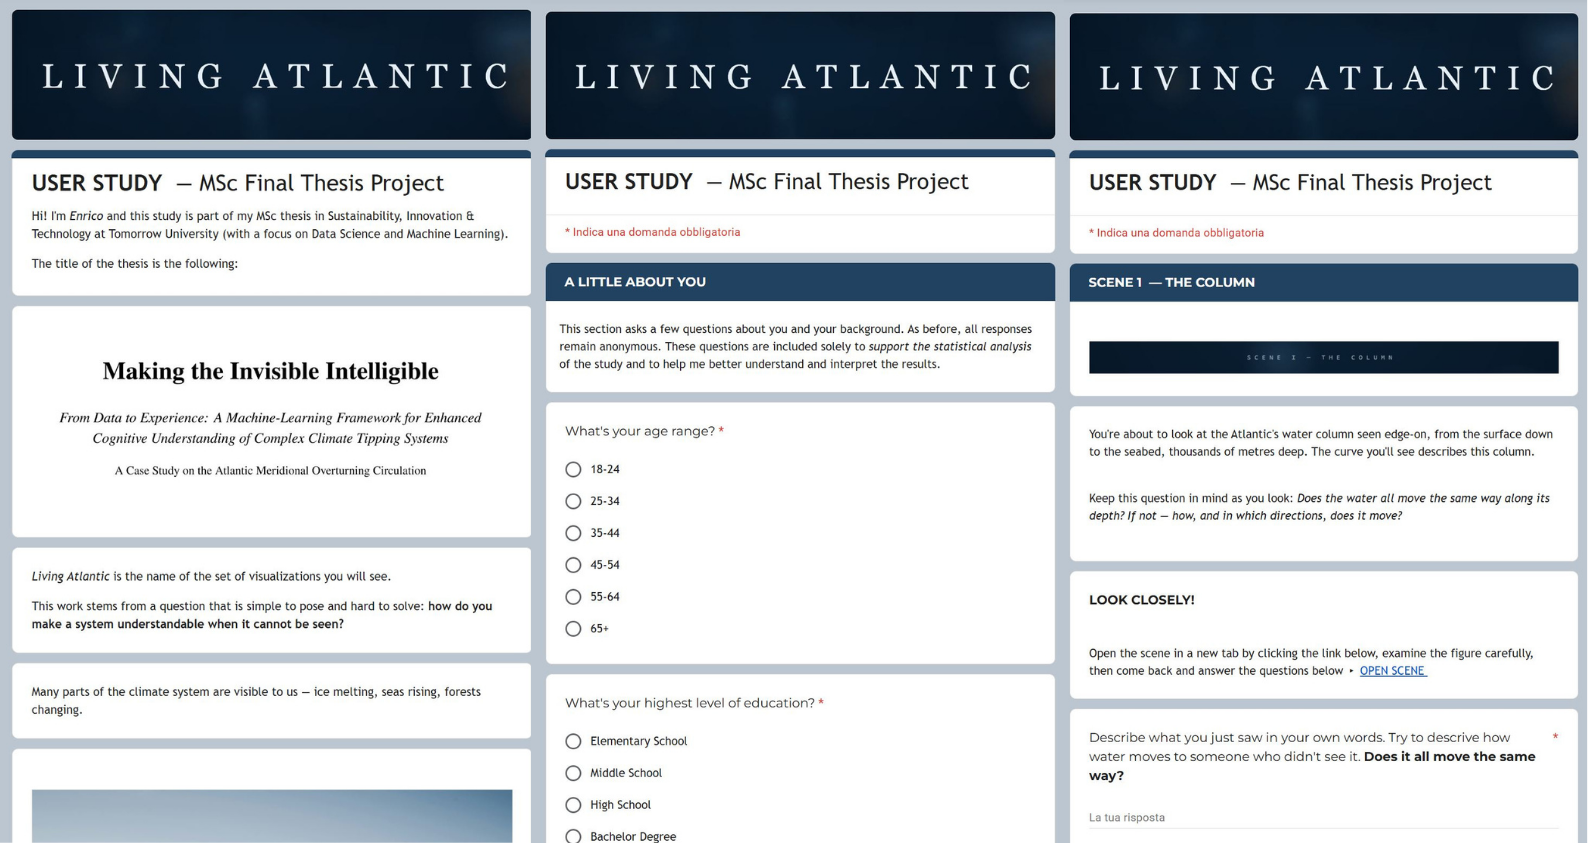
\includegraphics[width=\textwidth]{figures/user_study/Google_Form.png}
    \caption[Google Form]{Google Form used for data collection. The form was designed to collect participants' feedback on the proposed approach, including their experience with the system, perceived usability, and suggestions for improvement.}
    \label{fig:google-form}
\end{figure}

An earlier version of the study considered a think-aloud protocol with live sessions. This approach was later replaced by a written, self-administered survey. The written format makes it possible to reach more participants and gives everyone the same instructions and questions without the presence of an interviewer influencing their responses. This was considered more appropriate for the exploratory study and its relatively small sample.

The survey follows a single sequence: introduction, consent, anonymity information, a short background section, and the basic context needed to understand the AMOC and the sverdrup --- all identical for both groups. The three scenes then follow in order (\textit{The Column}, \textit{The Engine Room}, \textit{The Threshold}). For each, participants receive a short introduction and a guiding question, open the assigned visualisation in a new tab, explore it, and on returning answer a series of open questions in their own words. A final reflection and debrief close the survey.

The order of the questions is intentional: participants describe what they understood in their own words before being asked to rate their confidence or reflect on the experience, and the two-condition structure is explained only after the main responses have been collected.

% -------------------------------------------------------------------------
\section{Conditions of the Study}
\label{sec:eval-conditions}

The two groups differed only in the type of visualisation they experienced. Both saw the same three scenes --- \textit{The Column}, \textit{The Engine Room} and \textit{The Threshold} --- with the same questions and the same contextual information; the control group saw each as a conventional static visualisation, the experiential group as its interactive and dynamic counterpart.\footnote{The design of the three scenes, and the distinction between their machine-learning-derived and classical components, is described in \S\ref{sec:three-scenes}. Chapter~\ref{ch:translate} establishes that both conditions use the same data bundle, reconstruction function and provenance.}

One clarification matters for how the comparison should be read. Machine learning does not generate every element of the experiential visualisations: its role differs between scenes, and several elements are classical --- the particle field in Scene~I is a derivative, the ensemble spread in Scene~III comes from external ocean models. The study therefore compares two ways of presenting the same underlying system, not a machine-learning condition against a non-machine-learning one.

% -------------------------------------------------------------------------
\section{Randomisation and the Debrief}
\label{sec:eval-randomisation}

Participants were randomly assigned to one of the two conditions. With a small sample, randomisation cannot guarantee balanced groups, but it removes self-selection into a condition and so limits one systematic source of bias. Each participant stayed in their assigned condition to the end of the main study, so that exposure to the alternative could not influence their responses.\footnote{Keeping the experimental structure undisclosed until the end also reduces the possibility that participants interpret their experience as part of a comparison and adjust their responses accordingly.}

Once all main responses had been collected, the debrief explained the structure, introduced the two conditions, and gave every participant access to the complete set of visualisations --- including the version they had not experienced.

% -------------------------------------------------------------------------
\section{Background Section}
\label{sec:eval-demographics}

A short background section was included before the visualisation tasks. It collected information about age range, education, field of study or work, and self-rated familiarity with climate science, the AMOC and data visualisations.

The purpose of this section is mainly descriptive. Given the small sample size, these variables are not used as a basis for statistical modelling. Instead, they provide information about the participants and help describe the audience included in the study.

The demographic information therefore provides context for the results rather than acting as a separate analytical component.

% -------------------------------------------------------------------------
\section{Consent, Anonymity and Ethics}
\label{sec:eval-ethics}

Participation was voluntary and anonymous: the survey collected no names, email addresses or other direct identifiers, participants could stop at any point without giving a reason, and consent was obtained before the study began through an explicit confirmation that continuing meant agreeing to participate. Responses were used only for this research, and no identifying information appears in Chapter~\ref{ch:results}. The consent text, the anonymity statement and the data-management detail are reproduced in Appendix~\ref{app:protocols}; the ethical commitments they implement are set out in \S\ref{sec:ethics-statement} and Appendix~\ref{app:ethics-conduct}.

% -------------------------------------------------------------------------
\section{Evaluation Framework}
\label{sec:eval-framework}

The open responses are analysed against a predefined coding grid. The aim is not to mark answers right or wrong but to identify whether participants express the main structural idea each scene represents.\footnote{The complete grid, including the target for each scene and the definition of each category, is provided in Appendix~\ref{app:protocols}.}

The categories were defined before the responses were analysed, and each is tied to the driving question of its scene (\S\ref{sec:three-scenes}): opposing directions at different depths for Scene~I, recurrence between states for Scene~II, and change in the level of agreement between the three models for Scene~III. A response counts as showing understanding only when the participant describes the relevant structure in their own words; mentioning movement, colour or other visual features is not sufficient.

The coding was carried out through an assisted procedure. A large language model, instructed on the coding grid and its category definitions, produced an initial label for each response. The researcher then reviewed every label and corrected it wherever their own judgement differed from the automatic proposal. The final coding is therefore the result of human adjudication, with the automated pass serving only as a starting point.\footnote{The pre-defined coding grid (Appendix~\ref{app:protocols}) is what keeps this procedure transparent: each label can be rechecked by others using the fixed criteria and the original responses. No inter-coder agreement coefficient is reported, as this measure does not apply to a single-coder design supported by an automated first pass. The limitation of single-coder analysis is discussed in \S\ref{sec:eval-limitations}.}

The framework also keeps demonstrated understanding --- the written description --- separate from perceived understanding, the confidence rating, because participants may feel confident even when their interpretation does not match the intended structure.\footnote{\textcite{fischer2020} documents cases in which high confidence accompanies an incorrect interpretation. The analysis therefore cross-tabulates confidence against the coded responses rather than treating it as evidence of correct understanding.} The survey cannot measure everything a participant understands; it can only analyse what they communicate.

% -------------------------------------------------------------------------
\section{What the Study Expects to Find}
\label{sec:eval-expectations}

The study investigates whether the experiential condition may support a clearer understanding of system behaviour than the static condition, in the terms expectations E3.1 and E3.2 set out in \S\ref{sec:hypotheses}. Scene by scene: the experiential representation may make the relationship between depth and opposing directions easier to understand (Scene~I), recurrence between states easier to recognise (Scene~II), and changes in model agreement easier to perceive over time (Scene~III). These are expectations rather than predictions, and neither presumes a direction or magnitude of effect. The results are reported in Chapter~\ref{ch:results}.

% -------------------------------------------------------------------------
\section{Timing and Burden}
\label{sec:eval-burden}

The survey was designed to take fifteen to twenty minutes: short enough to avoid unnecessary fatigue, long enough to explore three visualisations. Participants could stop at any point.

% -------------------------------------------------------------------------
\section{Limitations of the Design}
\label{sec:eval-limitations}

The study has several important limitations. First, the sample is small, with twenty-five participants in total. The two groups are also slightly unbalanced, with twelve participants in the static condition and thirteen in the experiential condition. The sample size does not provide sufficient statistical power for strong inferential analysis or population-level generalisation.

Second, participants were recruited through personal networks, making the sample one of convenience. Its age, background and experience may therefore differ from those of the wider population that the visualisations are ultimately intended to reach.

Third, all participants met the three scenes in the same fixed order (I, II, III), chosen for the interpretive reasons set out in \S\ref{sec:three-scenes}. Because that order was not counterbalanced, position in the sequence is confounded with scene identity: any comparison \emph{between} scenes carries a possible contribution from learning across the sequence or from fatigue toward its end. This bears directly on the Scene~III result, where the experiential condition performed less well and where the task also fell last in a fifteen- to twenty-minute survey. Counterbalancing scene order is a requirement for any larger replication.

Fourth, the study uses written and self-reported responses. This means that the analysis is limited to what participants are able or willing to express in writing. Some aspects of understanding may therefore remain unobserved.

Fifth, the responses were coded by a single researcher, supported by an automated first pass and without an independent second coder. No inter-coder reliability can therefore be reported, and the automated pass introduces a specific risk of its own: a human reviewer who sees a proposed label first may anchor on it rather than judging the response independently. The pre-specified coding grid mitigates both limitations by keeping each assignment open to external rechecking against fixed criteria, but it does not fully replace independent double coding.

Sixth, the two conditions place different demands on the participant's hardware. The experiential condition renders in WebGL with real-time audio and the static condition does not, so a slower device degrades one condition and not the other. No device or browser information was collected, and this asymmetry is therefore acknowledged rather than controlled.

Finally, the study distinguishes between demonstrated and perceived understanding. A participant may report high confidence without showing the expected structural understanding in their written response. This is not treated as a methodological error, but as an important distinction that the evaluation framework is designed to capture.

% (Google_Form.tex was here, orphaned after the last section; it now sits in 8.4)
These limitations do not remove the value of the study. The purpose of this work is to provide a first empirical test of the approach and to identify patterns that can guide future research. A larger and more controlled study would be needed to test the findings with greater statistical power. The present study therefore provides an initial empirical foundation rather than a final validation of the proposed approach.